%
% This is a borrowed LaTeX template file for lecture notes for CS267,
% Applications of Parallel Computing, UCBerkeley EECS Department.
% Now being used for CMU's 10725 Fall 2012 Optimization course
% taught by Geoff Gordon and Ryan Tibshirani.  When preparing 
% LaTeX notes for this class, please use this template.
%
% To familiarize yourself with this template, the body contains
% some examples of its use.  Look them over.  Then you can
% run LaTeX on this file.  After you have LaTeXed this file then
% you can look over the result either by printing it out with
% dvips or using xdvi. "pdflatex template.tex" should also work.
%

\documentclass[twoside]{article}
\setlength{\oddsidemargin}{0.25 in}
\setlength{\evensidemargin}{-0.25 in}
\setlength{\topmargin}{-0.6 in}
\setlength{\textwidth}{6.5 in}
\setlength{\textheight}{8.5 in}
\setlength{\headsep}{0.75 in}
\setlength{\parindent}{0 in}
\setlength{\parskip}{0.1 in}

%
% ADD PACKAGES here:
%

\usepackage{amsmath,amsfonts,graphicx}

%
% The following commands set up the lecnum (lecture number)
% counter and make various numbering schemes work relative
% to the lecture number.
%
\newcounter{lecnum}
\renewcommand{\thepage}{\thelecnum-\arabic{page}}
\renewcommand{\thesection}{\thelecnum.\arabic{section}}
\renewcommand{\theequation}{\thelecnum.\arabic{equation}}
\renewcommand{\thefigure}{\thelecnum.\arabic{figure}}
\renewcommand{\thetable}{\thelecnum.\arabic{table}}

%
% The following macro is used to generate the header.
%
\newcommand{\lecture}[4]{
   \pagestyle{myheadings}
   \thispagestyle{plain}
   \newpage
   \setcounter{lecnum}{#1}
   \setcounter{page}{1}
   \noindent
   \begin{center}
   \framebox{
      \vbox{\vspace{2mm}
    \hbox to 6.28in { {\bf ROB501 - Fundamentals \& Emerging Topics in Robotics - Digital Control Systems } }
       \vspace{4mm}
       \hbox to 6.28in { {\Large \hfill Lecture #1 \hfill} }
       \vspace{2mm}
       \hbox to 6.28in { {\it Lecturer: #2 \hfill } }
      \vspace{2mm}}
   }
   \end{center}
   \markboth{Lecture #1}{Lecture #1}

   \vspace*{4mm}
}
%
% Convention for citations is authors' initials followed by the year.
% For example, to cite a paper by Leighton and Maggs you would type
% \cite{LM89}, and to cite a paper by Strassen you would type \cite{S69}.
% (To avoid bibliography problems, for now we redefine the \cite command.)
% Also commands that create a suitable format for the reference list.
\renewcommand{\cite}[1]{[#1]}
\def\beginrefs{\begin{list}%
        {[\arabic{equation}]}{\usecounter{equation}
         \setlength{\leftmargin}{2.0truecm}\setlength{\labelsep}{0.4truecm}%
         \setlength{\labelwidth}{1.6truecm}}}
\def\endrefs{\end{list}}
\def\bibentry#1{\item[\hbox{[#1]}]}

%Use this command for a figure; it puts a figure in wherever you want it.
%usage: \fig{NUMBER}{SPACE-IN-INCHES}{CAPTION}
\newcommand{\fig}[3]{
			\vspace{#2}
			\begin{center}
			Figure \thelecnum.#1:~#3
			\end{center}
	}
% Use these for theorems, lemmas, proofs, etc.
\newtheorem{theorem}{Theorem}[lecnum]
\newtheorem{lemma}[theorem]{Lemma}
\newtheorem{proposition}[theorem]{Proposition}
\newtheorem{claim}[theorem]{Claim}
\newtheorem{corollary}[theorem]{Corollary}
\newtheorem{definition}[theorem]{Definition}
\newenvironment{proof}{{\bf Proof:}}{\hfill\rule{2mm}{2mm}}

% **** IF YOU WANT TO DEFINE ADDITIONAL MACROS FOR YOURSELF, PUT THEM HERE:

\begin{document}

% Lecture Details
\lecture{6}{Asst. Prof. M. Mert Ankarali}


\section{Root Locus in Discrete-Time \& Digital Control Systems}

For continuous time systems the root locus diagram illustrates the
location of roots/poles of a closed loop LTI systems, with respect 
to gain parameter $K$ (can be considered as a P controller). The
basic closed-loop topology is used for deriving the root-locus
rules, however we know that many different topologies can be reduced
to this from.

\begin{center}
\begin{minipage}[h]{0.7\linewidth}
    \begin{center}
      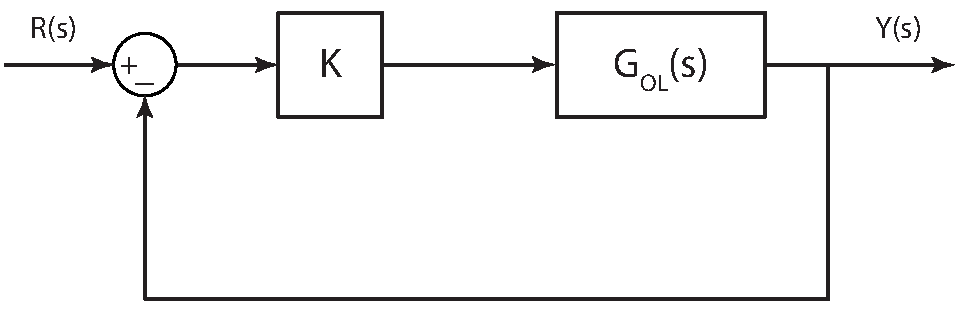
\includegraphics[width=\textwidth]{cont}
    \end{center}
\end{minipage}
\end{center}

The closed loop transfer function of this basic control system is
%
\begin{align*}
\frac{Y(s)}{R(s)} = \frac{K G_{OL}(s)}{1 + K G_{OL}(s)}
\end{align*}
%
where the poles of the closed loop system are
the roots of the characteristic equation 
%
\begin{align*}
1 + K G_{OL}(s) = 0 
\\
1 + K \frac{n(s)}{d(s)} = 0 
\end{align*}
%
In 302 we learned the rules such that we can derive the
qualitative and quantitive structure of root locus paths
for \textbf{positive} gain $K$ that solves the equation
above.

In discrete time systems, similar to the CT case 
we use the root locus diagram to illustrate the
location of roots/poles of a closed loop DT-LTI systems, with respect 
to a gain parameter $K$ (can be considered as a P controller). The
basic discrete-time closed-loop topology is used for deriving the root-locus
rules, however we know that many different DT topologies can be reduced
to this from.

\begin{center}
\begin{minipage}[h]{0.7\linewidth}
    \begin{center}
      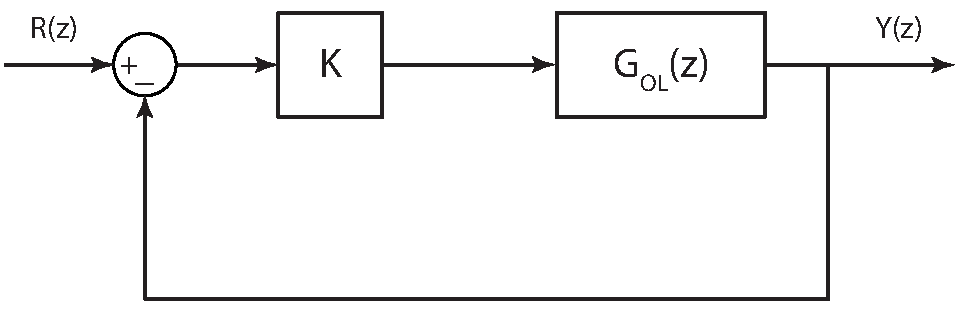
\includegraphics[width=\textwidth]{dist}
    \end{center}
\end{minipage}
\end{center}

The closed loop transfer function of this basic control system is
%
\begin{align*}
\frac{Y(z)}{R(z)} = \frac{K G_{OL}(z)}{1 + K G_{OL}(z)}
\end{align*}
%
where the poles of the closed loop system are
the roots of the characteristic equation 
%
\begin{align*}
1 + K G_{OL}(z) = 0 
\\
1 + K \frac{n(z)}{d(z)} = 0 
\end{align*}
%
I think, it is obvious that fundamental 
equation that relates the gain $K$ and roots/poles
is exactly same for both CT and DT systems.
This means that same rules are directly applied 
for CT systems. 

However, even if we have same diagram for CT and DT 
systems the meaning and interpretation of the diagram
is fundamentally different. Because, the effects of pole 
locations are different in CT and DT systems. 

\subsection*{Angle and Magnitude Conditions}

Let's analyze the characteristic equation 
%
\begin{align*}
K G_{OL}(z) = -1 \quad , &\mathrm{or} \quad K \frac{n(z)}{d(z)} = -1 
\\
| K G_{OL}(z) | = 1 \quad , &\mathrm{or} \quad \left| K \frac{n(z)}{d(z)} \right| = 1 
\\
\angle [ K G_{OL}(z) ] = \pi (2 k + 1) , \ k \in \mathbb{Z} \quad ,
  &\mathrm{or} \quad \angle \left[ K \frac{n(z)}{d(z)} \right] = \pi (2 k + 1), \ k \in \mathbb{Z} 
\end{align*}
%
For a given $K$, z values that satisfy both magnitude and angle
conditions are located on the root loci.

\subsection*{Rules and procedure for constructing root loci}

\begin{enumerate} 

\item Characteristic equation, zeros and poles of the
  Open-Loop pulse transfer function.
%
\begin{align*}
1 + K G_{OL}(z)  &= 0 \\
1 + K \frac{n(z)}{d(z)} &= 0 \\
1 + K \frac{(z - z_1) \cdots (z - z_M)}{(z - p_1) \cdots (z - p_N)} &= 0 \\
\end{align*}
%

\item Root loci has $N$ separate branches. 

\item Root loci starts from poles of $G_{OL}(z)$ and 
%
\begin{enumerate} 
   \item $M$ branches terminates at the zeros of $G_{OL}(z)$
   \item $N-M$ branches terminates at $\infty$ (implicit zeros of $G_{OL}(z)$)
\end{enumerate}

It is relatively easy to undestand this 
%
\begin{align*}
d(z) + K n(z) = 0 
\\
K \to 0 \ \rightarrow \ d(z) = 0
\\
K \to \infty \ \rightarrow \ n(z) = 0
\end{align*}

\item Root loci on the real axis determined by open-loop zeros and
  poles. $z = \sigma \in \mathbb{R}$ then, 
%
\begin{align*}
| K G_{OL}(\sigma) | &= 1
\\
\mathrm{Sign} [ G_{OL}(\sigma) ] &= -1
\end{align*}
%
We can always find a $K$ that satisfy the magnitude condition, so
angle condition will determine which parts of real axis belong to the
root locus.

We can first see that complex conjugate zero/pole pairs has not effect, then for
the remaining ones we can derive the following condition
%
\begin{align*}
\mathrm{Sign} [ G_{OL}(\sigma) ] = \prod_{i=1}^M  \mathrm{Sign} [\sigma - z_i]
  \prod_{j=1}^N  \mathrm{Sign} [\sigma - p_j] = -1
\end{align*}
%
which means that for ODD number of poles $+$  zeros 
$\mathrm{Sign} [\sigma - p_i ]$ and $\mathrm{Sign} [\sigma - z_i] $ 
must be negative for satisfying this condition for that particular $\sigma$
to be on the root-locus. We can summarize the rule as

\textbf{If the test point $\sigma$ on real axis has ODD numbers of 
poles and zeros in its right, then this point is located 
on the root-locus.}

\item Asymptotes

\begin{itemize}
  \item $N-M$ branches goes to infinity. Thus, there exist $N-M$ many
    asymptotes
  \item For large $z$ we can have the following approximation
 \begin{align*}
  &K \frac{(z - z_1) \cdots (z - z_M)}{(z - p_1) \cdots (z - p_N)}
   \approx \frac{K}{z^{N-M}}
\\
&\angle \left[ \frac{K}{z^{N-M}} \right] = -(N-M) \angle [ z ] = \pi (2 k + 1), \ k \in \mathbb{Z} 
\\
&\phi_{a} = \frac{\pm \pi (2 k + 1)}{N-M}, \ k \in \lbrace 1, \cdots, N-M \rbrace
 \end{align*}
%
  \item Real axis intercept $\sigma_a$ can be computed as
 \begin{align*}
   \sigma_a = \frac{\sum p_i - \sum z_i}{N-M}
 \end{align*}
%
This can be derived via a different approximation (see textbook)
\end{itemize}

\item Breakaway and break-in points on real axis. When z is real 
$z = \sigma, \ \sigma \in \mathbb{R}$, we can have
%
\begin{align*}
1 + K G_{OL} (\sigma) = 0 \quad \rightarrow \quad K(\sigma) =
  \frac{-1}{G_{OL} (\sigma) }
\end{align*}
%
Note that break-in and breakaway points corresponds to 
double roots. Thus, $\sigma_{b}$ is a break-away or break-in 
point if 
%
\begin{align*}
\left[ \frac{d K(\sigma)}{d \sigma} \right]_{\sigma = \sigma_b} &= 0
                                                                \quad
                                                                \mathrm{or}
                                                                \quad
                                                                \left[
                                                                  \frac{d
                                                                  G_{OL}(\sigma)}{d
                                                                  \sigma} \right]_{\sigma = \sigma_b} = 0
\\
K(\sigma) > 0
\end{align*}
%


\item Angle of departure (or arrival) from open-loop complex 
conjugate poles (or to open-loop complex conjugate zeros)

Let's assume that $p^*$ is a complex conjugate pole of $G_{OL}(z)$, then let's define a
$P(z)$ such that
%
\begin{align*}
  P^*(z) = (z - p^*) G_{OL}(z)
\end{align*}
%
We know that for $K = 0$, the root locus is located at $p^*$. If we
add a very small $K = \delta K$, then pole/root locus moves to $p^* +
\delta z$. If we evaluate the phase condition of the root locus on
this new ``unknown'' point
%
\begin{align*}
\angle [ K G_{OL}(z) ]_{z = p*+\delta z} &= \pm \pi 
\\
\angle \left[  \frac{P^*(z)}{z - p^*} \right]_{z = p^* + \delta z} &=
                                                                    \pm
                                                                     \pi
\\
\angle \left[  P^*(p^* + \delta z) \right]
-
\angle \left[ \delta z \right] &= \pm \pi
\\
\theta_{d} = \angle \left[ \delta z \right] &= \pm \pi + \angle \left[  P^*(p^*) \right]
\end{align*}

Geometrically speaking, $\angle \left[  P^*(p^*) \right]$ stands for
\textbf{\# of angles from the zeros to this specific pole
  $-$ \# of angles from all other remaining poles to this specific pole}.

A similar condition can be derived for angle of arrival to complex
conjugate zeros.
%
\begin{align*}
\theta_{a} &= \pm \pi - \angle \left[  P^*(z^*) \right]
\\
P^*(z) &= (z - z^*) G_{OL}(z)
\end{align*}
%
where $z^*$ is a complex conjugate zero of $G_{OL}(z)$.

\end{enumerate}

\newpage

\textbf{Examples}

\begin{minipage}[h]{0.5\linewidth}
    \begin{center}
      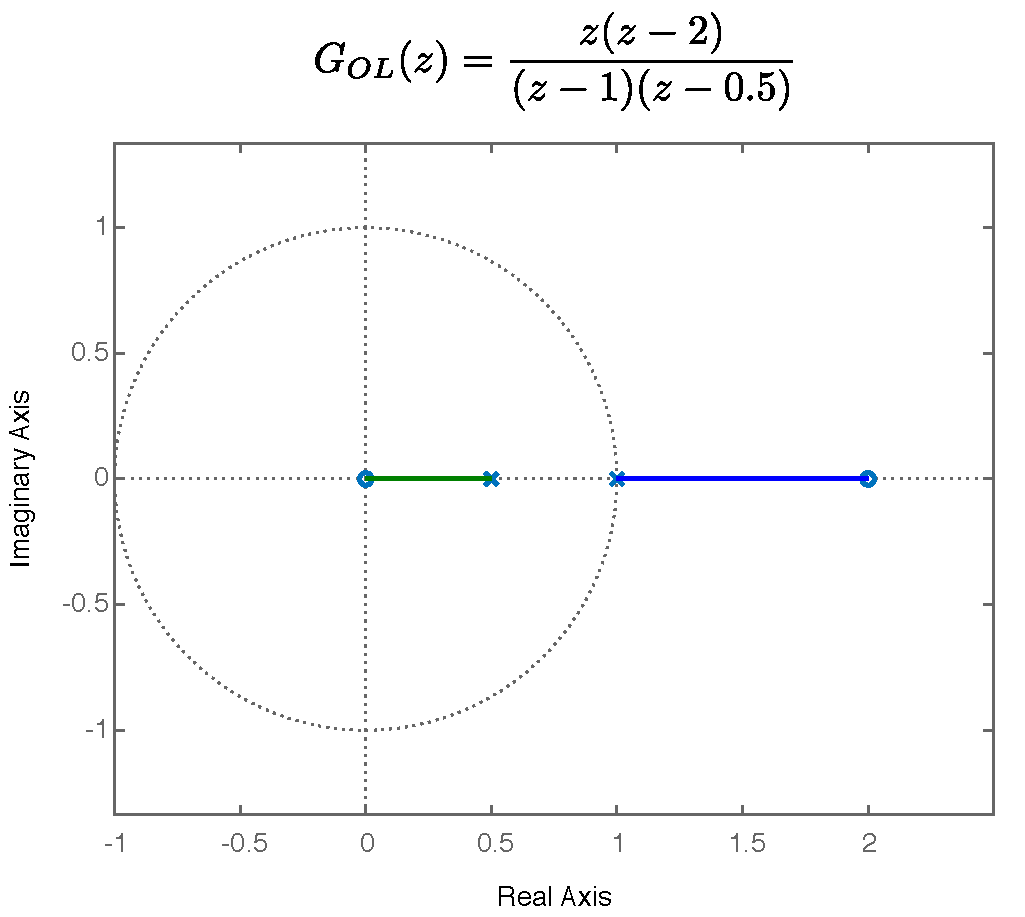
\includegraphics[width=0.95\textwidth]{E1}
    \end{center}
\end{minipage}
\begin{minipage}[h]{0.5\linewidth}
    \begin{center}
      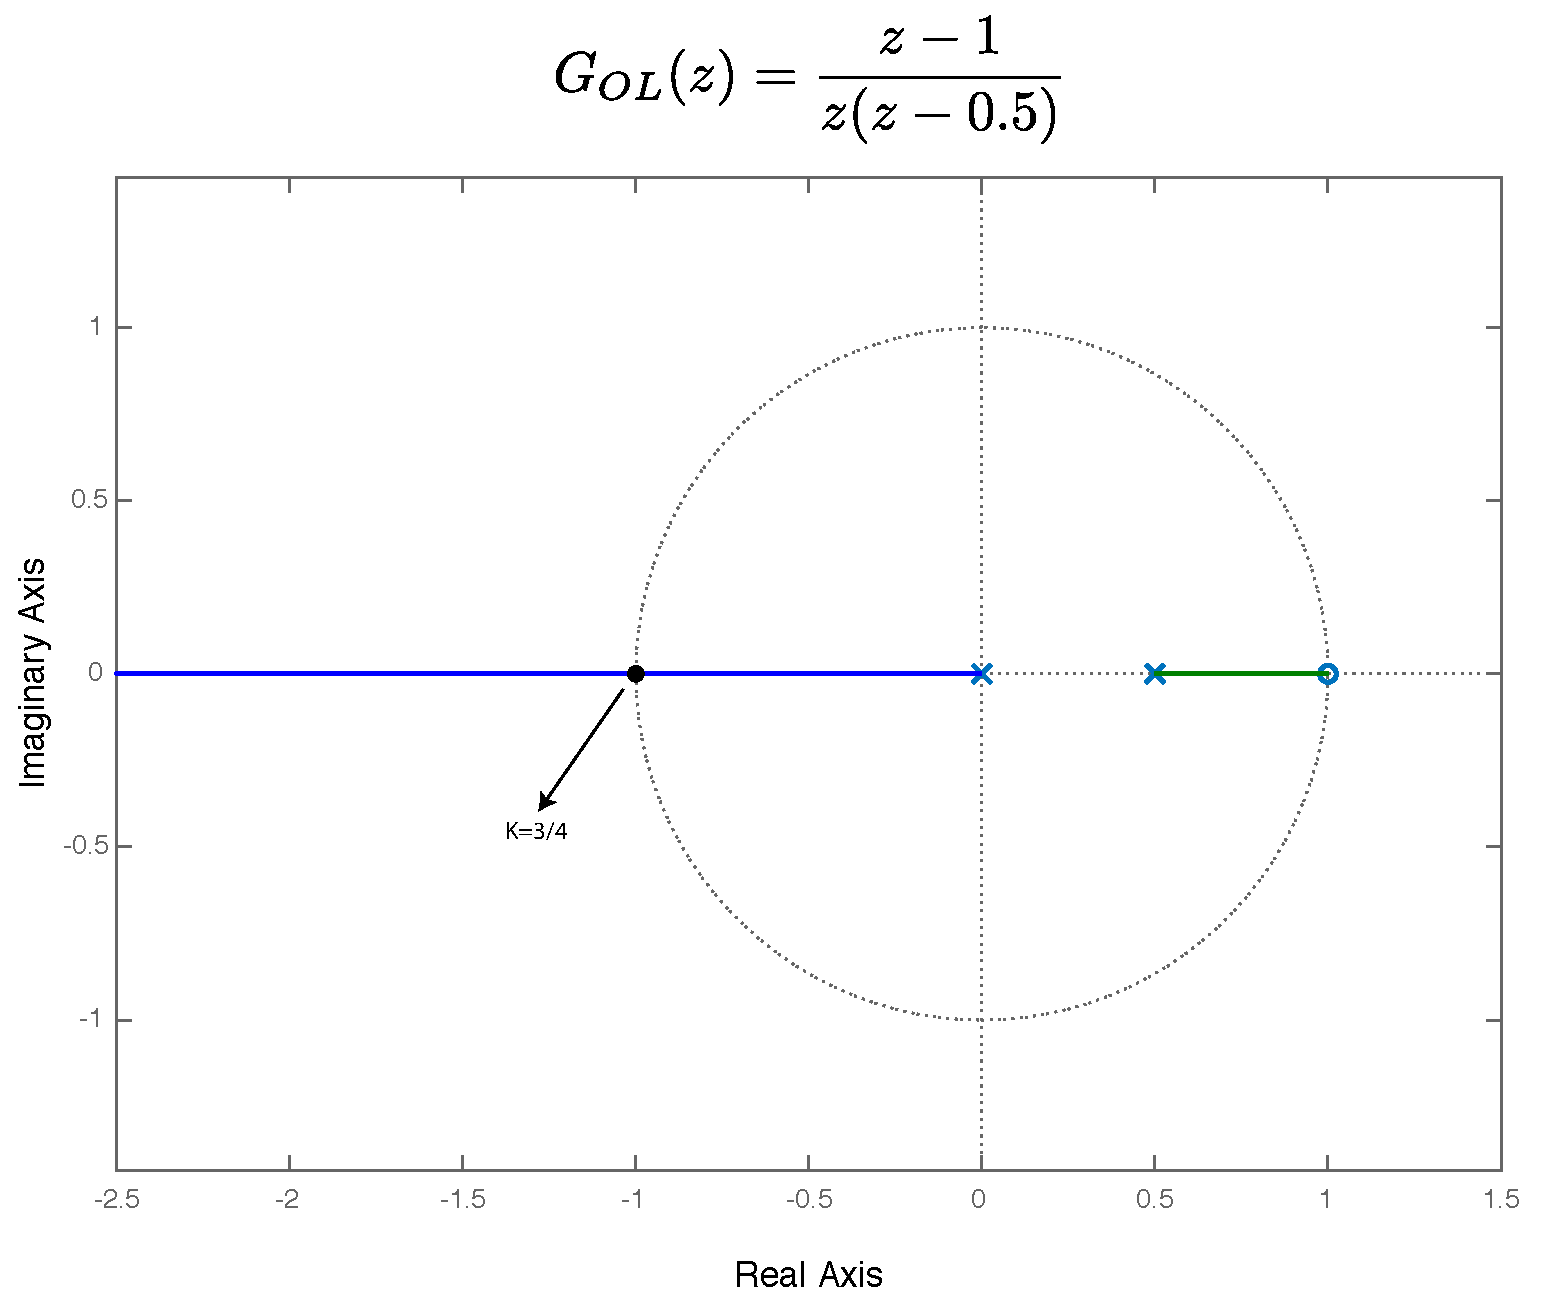
\includegraphics[width=0.95\textwidth]{E2}
    \end{center}
\end{minipage}

\begin{center}
\begin{minipage}[h]{\linewidth}
    \begin{center}
      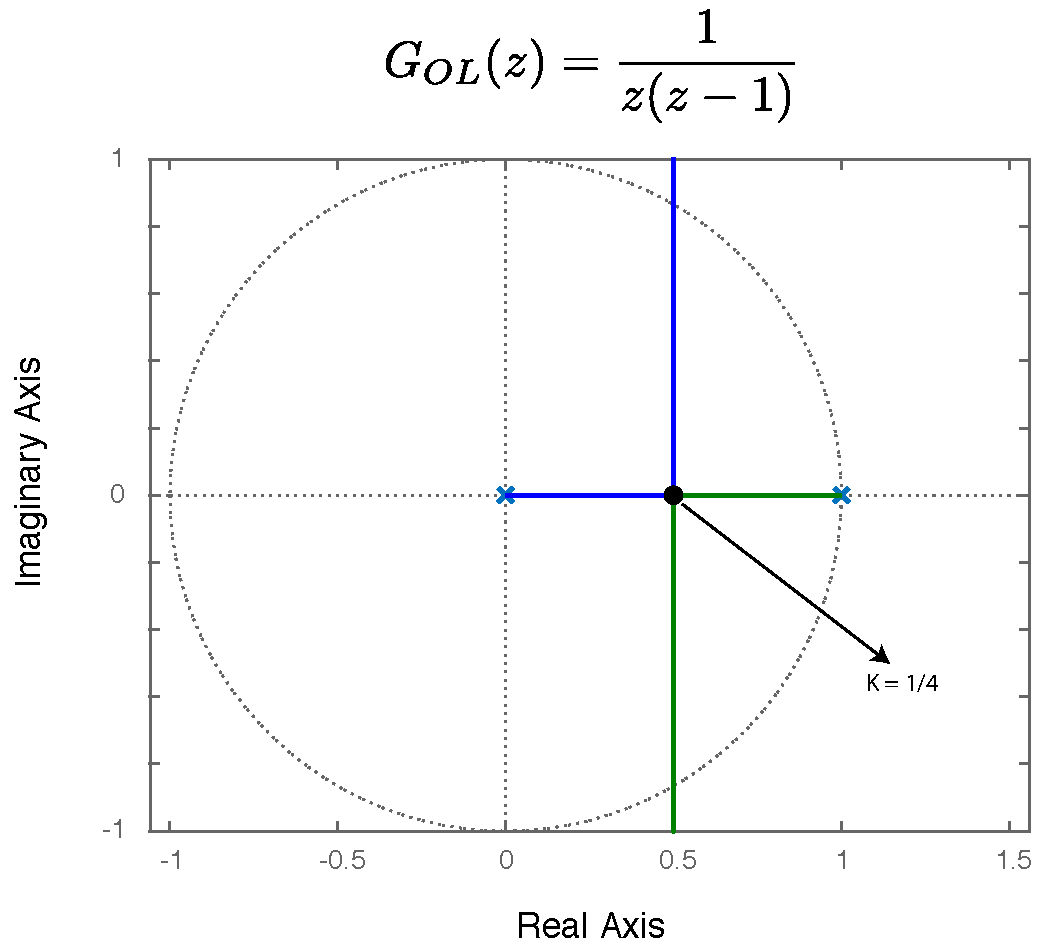
\includegraphics[width=0.65\textwidth]{E3}
    \end{center}
\end{minipage}
    \end{center}

\begin{center}
\begin{minipage}[h]{\linewidth}
    \begin{center}
      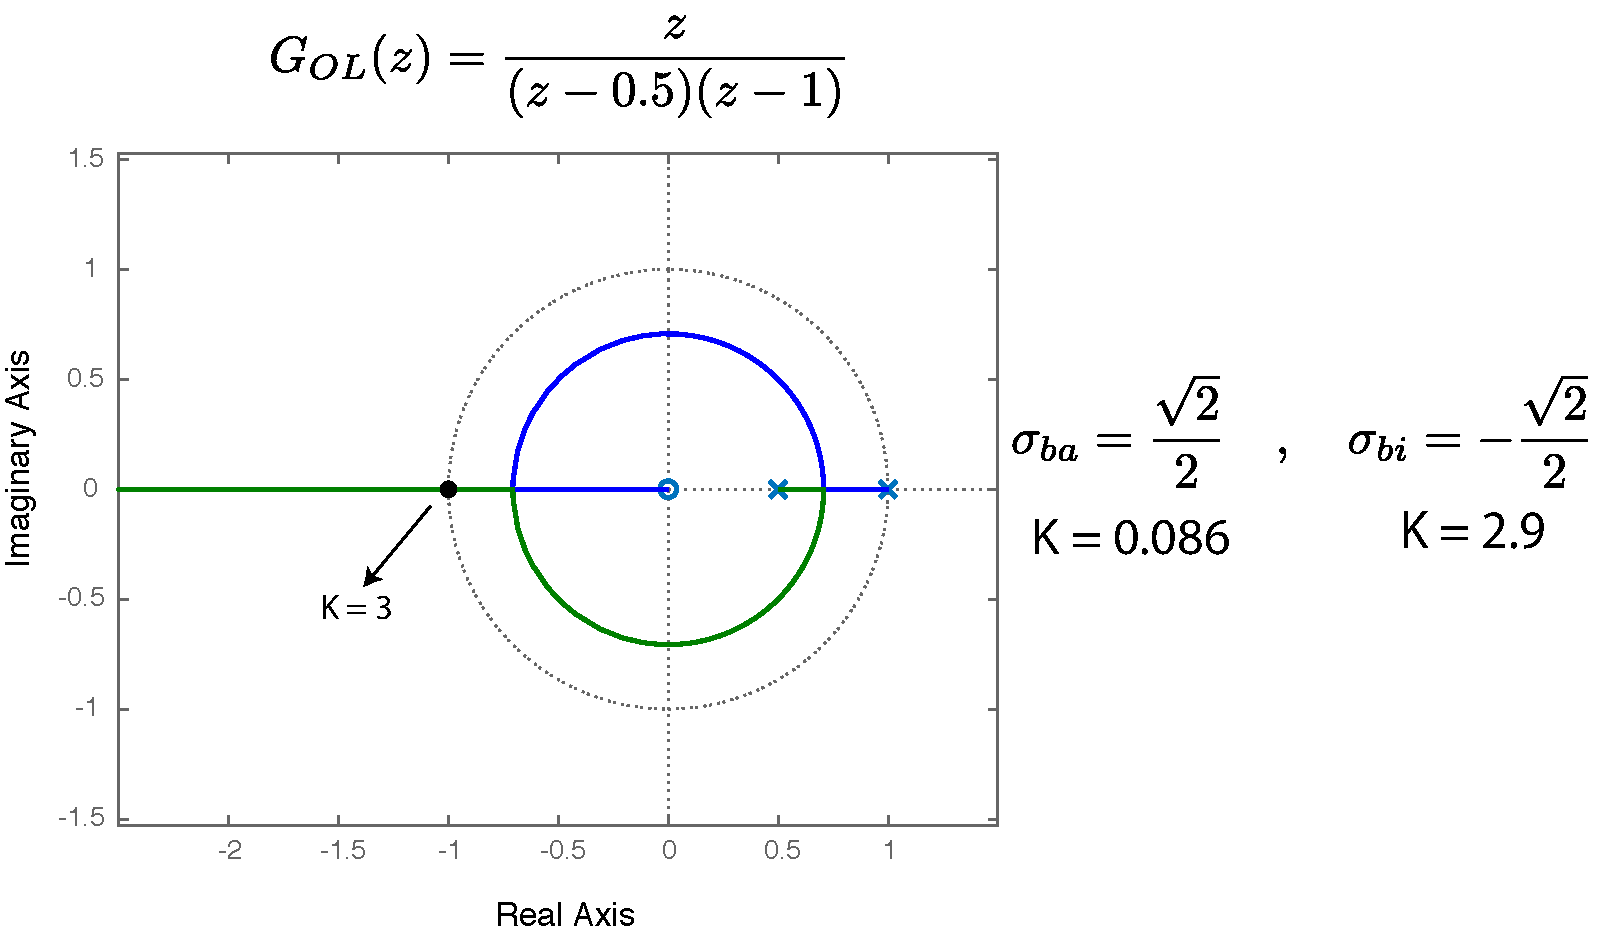
\includegraphics[width=0.95\textwidth]{E4}
    \end{center}
\end{minipage}
    \end{center}

\begin{center}
\begin{minipage}[h]{\linewidth}
    \begin{center}
      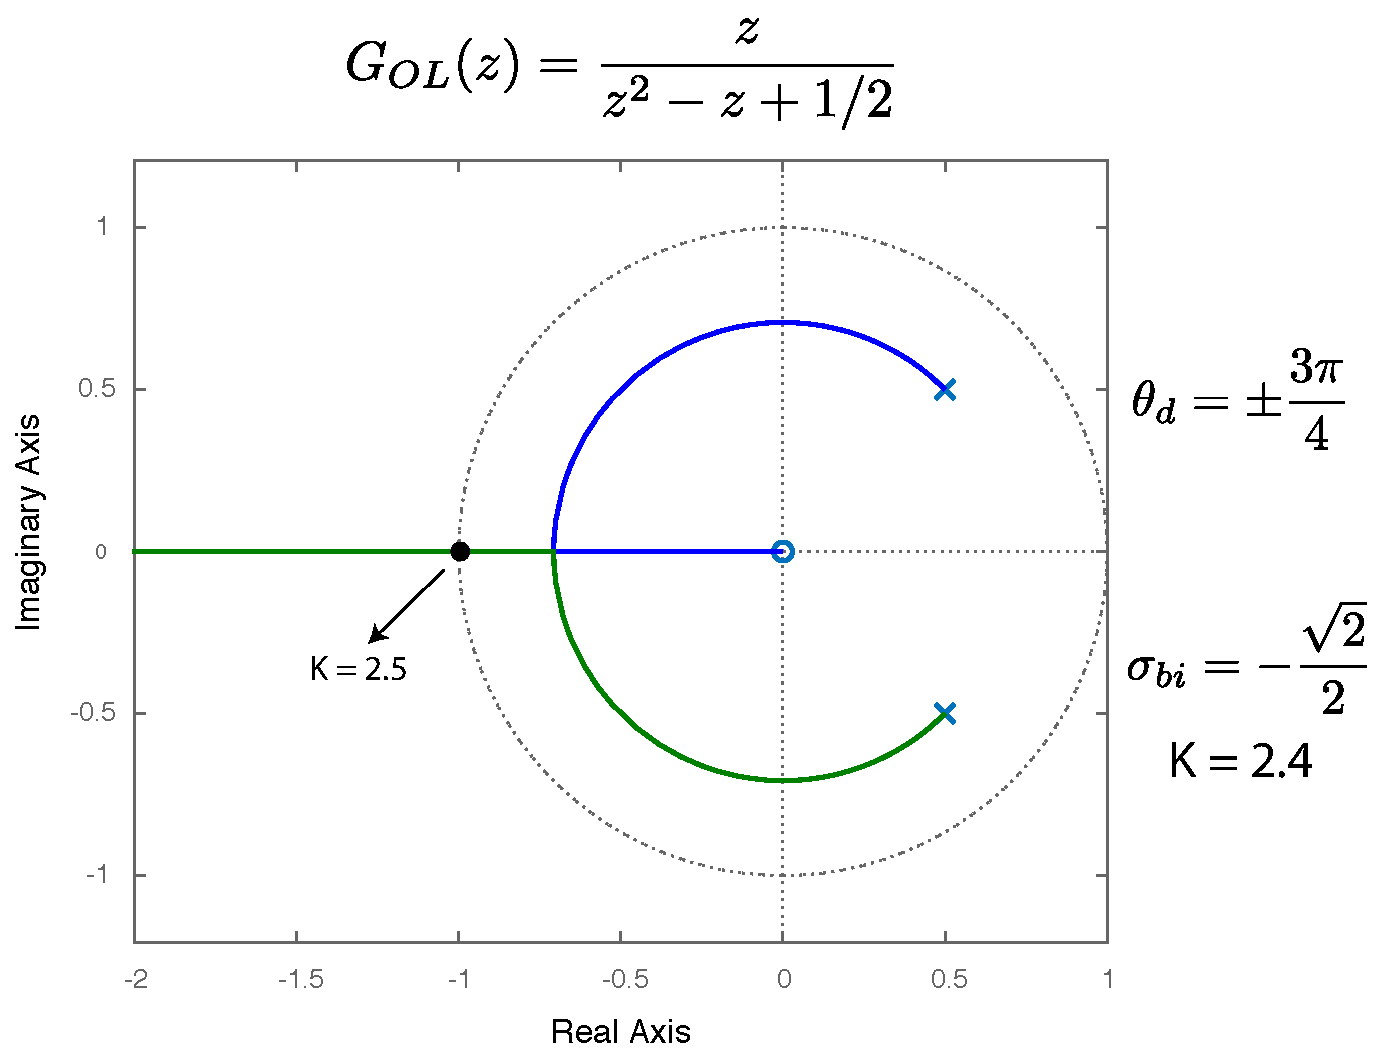
\includegraphics[width=0.7\textwidth]{E5}
    \end{center}
\end{minipage}
    \end{center}

\newpage

\subsection{Root-locus with respect to different parameters}

Let's consider the following discrete-time system where the plant has a 
transfer function of $G(z)$ and controller is a first-order FIR filter
(low-pass) with a transfer function of  $G_c(z) = 1/4 + A z^{-1}$.
We want to derive the location of closed-loop poles with respect to 
the parameter $A$, which does not directly fit to the classical form. 

\begin{center}
\begin{minipage}[h]{\linewidth}
    \begin{center}
      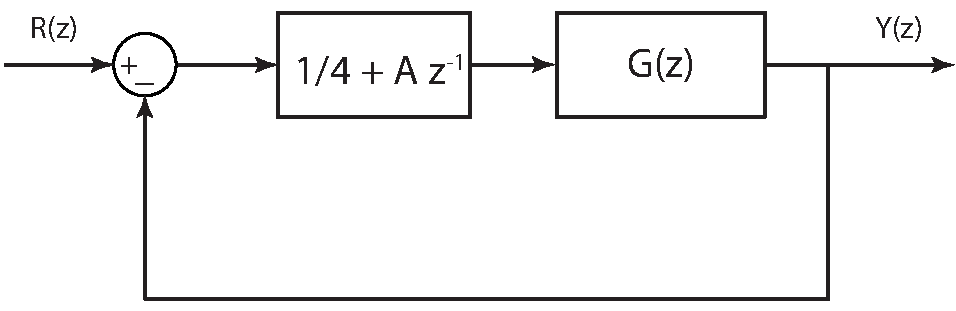
\includegraphics[width=0.6\textwidth]{distdiff}
    \end{center}
\end{minipage}
\end{center}

Let's first compute the closed-loop PTF and analyze the characteristic
equation.
%
\begin{align*}
  \frac{Y(z)}{R(z)} &= \frac{ \left(0.25 + A z^-1 \right) G(z) }{1 +
                      \left (0.25 + A z^-1 \right) G(z)} 
\\
1 + \left( 0.25 + A z^{-1} \right) G(z) &= 0
\\
1 + 0.25 G(z) + A z^{-1} G(z) &= 0
\end{align*}
%
If we divide the characteristic equation by $1 + 0.25 G(z)$ we obtain
%
\begin{align*}
1+ A \frac{z^{-1} G(z)}{1 + 0.25 G(z)} &= 0
\\
1+ A \bar{G}_{OL}(z) &= 0
\end{align*}
%
Now if we consider as $\bar{G}_{OL}(z)$ as the open-loop transfer
function and draw the root-locus then we would derive the dependence 
of the roots to the parameter A. 

Let's assume that $G(z) = \frac{1}{z(z-1)}$. Then for this
system, we can compute
%
\begin{align*}
  \bar{G}_{OL}(z) &= \frac{z^{-1} G(z)}{1 + 0.25 G(z)}
= \frac{\frac{1}{z^2(z-1)}}{1 + \frac{0.25}{z(z-1)}}
= \frac{\frac{1}{z^2(z-1)}}{\frac{z^2 - z + 0.25}{z(z-1)}}
\\
&= \frac{1}{z (z^2 -z + 0.25)}
\end{align*}

Root-locus of the system w.r.t parameter $A$ is given below. It
can be seen that as A increases, dominant system poles deviates
from the origin and eventually becomes unstable at $A = 0.5$.
Technically this is a simple low-pass filter which may be inevitable
in many closed-loop control systems. However, as we decrease 
the cut-off frequency (by increasing A) we push the poles towards 
the unit circle thus making the system less stable.

\begin{center}
\begin{minipage}[h]{\linewidth}
    \begin{center}
      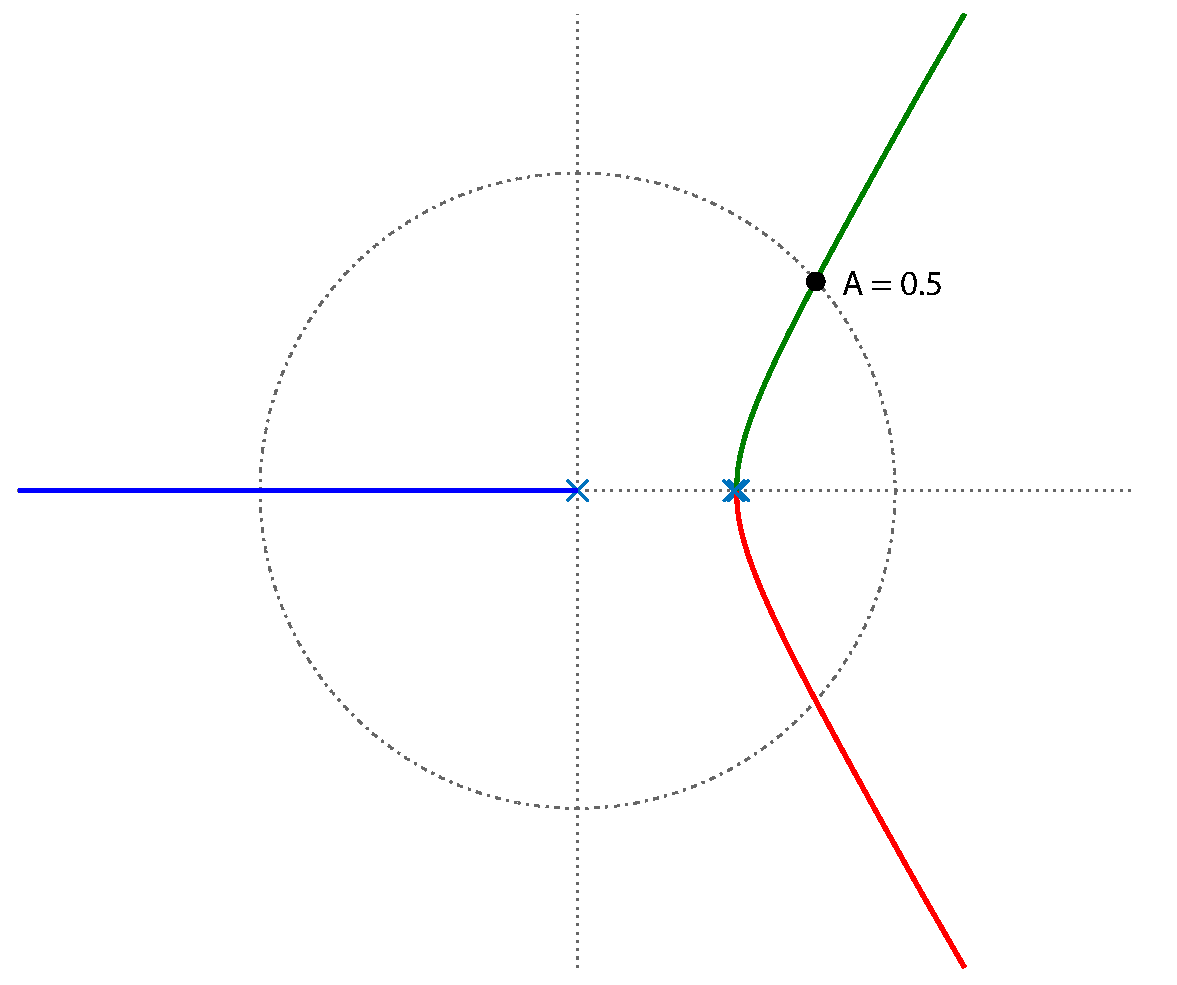
\includegraphics[width=0.6\textwidth]{rlocusA}
    \end{center}
\end{minipage}
\end{center}

% **** This ENDS THE EXAMPLES. DON'T DELETE THE FOLLOWING LINE:
\end{document}
